\documentclass[a4paper]{article}
\usepackage[utf8]{inputenc} % Skal passe til editorens indstillinger
\usepackage[english]{babel} % danske overskrifter


\newcommand{\name}{Carsten Nielsen}
%\newcommand{\stnumber}{s123369, s123161, s123821}
\newcommand{\course}{INI 404 Neuromorphic Engineering~I}
\newcommand{\university}{University of Zürich}
\newcommand{\studyline}{Institute of Neuroinformatics}
\newcommand{\assignment}{Lab 8 Post-Lab}
\renewcommand{\date}{\today} %If another date, than that of today is desiered


% Palatino for rm and math | Helvetica for ss | Courier for tt
\usepackage{mathpazo} % math & rm
\linespread{1.05}        % Palatino needs more leading (space between lines)
\usepackage{palatino} % tt
\normalfont
\usepackage[T1]{fontenc}
\usepackage[english]{babel}

\usepackage{graphicx}%allerese hentet % indsættelse af billeder
\usepackage{epstopdf} %Tilfj "--enable-write18" i argumentet for LaTex build. Dette vil konvertere .eps figurer til pdf-format
\graphicspath{{./picture/}} % stivej til bibliotek med figurer
\usepackage{subcaption} %Til gruppering af figurer
\usepackage{amsmath} %matpakke
\usepackage{amsfonts} %
\usepackage{amssymb} %
\usepackage{steinmetz} % flere matematik symboler
\usepackage{polynom} %for displaying polynom division
\usepackage{mathtools} % matematik - understøtter muligheden for at bruge \eqref{}
\usepackage{float}
\usepackage{placeins}
\usepackage{hhline}

%
\usepackage[usenames,dvipsnames]{xcolor}
\usepackage[compact,explicit]{titlesec}% http://ctan.org/pkg/titlesec
%
\usepackage[europeanresistors]{circuitikz}
\usepackage{pgfplots}
\usepgfplotslibrary{patchplots}
\pgfplotsset{compat=1.11}

%---------%
%Easy edit%
%---------%

%Section formating. arg1 is supplied when making section
\newcommand\presectionnumber[1]{~~}
\newcommand\postsectionnumber[1]{}
\newcommand\midlesection[1]{#1}
\newcommand\sectionnum[1]{\arabic{#1}}
\newcommand\subsectionnum[1]{\arabic{#1}}
\newcommand\subsubsectionnum[1]{\alph{#1}}



%------------%
%setion setup%
%------------%
\renewcommand\thesection{Opgave~\sectionnum{section}} %pas p�, kun i matematik
\renewcommand\thesubsection{\thesection,~\subsectionnum{subsection}}
\definecolor{MagRed}{RGB}{190,40,15}
\definecolor{MathGreen}{RGB}{82,164,0}

\titleformat{\section}{\normalfont\sffamily\large\bfseries\color{MathGreen}}{}{0pt}{|\kern-0.15ex|\kern-0.15ex|\kern-0.15ex|\presectionnumber{#1}\sectionnum{section}\postsectionnumber{#1}\qquad\quad\midlesection{#1}\label{sec:\sectionnum{section}}}
\titleformat{\subsection}[runin]{\large\bfseries}{}{10pt}{\sectionnum{section}.\subsectionnum{subsection})~#1\label{sec:\sectionnum{section}.\subsectionnum{subsection}}}
\titleformat{\subsubsection}[runin]{\itshape}{}{0pt}{\subsectionnum{subsection},\subsubsectionnum{subsection}~#1\label{sec:\sectionnum{section}.\subsectionnum{subsection}.\subsubsectionnum{subsubsection}}}
%\titleformat{\subsubsection}{\bfseries}{}{0pt}{\alph{subsection}.\arabic{subsubsection})\qquad\quad#1\label{\arabic{section}\alph{subsection}\arabic{subsubsection}}}

%----------%
%page setup%
%----------%
\textwidth = 400pt
\marginparwidth = 86pt
\hoffset = -25pt
\voffset= -30pt
\textheight = 670pt

%--------%
%hyperref%
%--------%
\newcommand{\HRule}{\rule{\linewidth}{0.5mm}}
\usepackage{fancyhdr}
\usepackage[plainpages=false,pdfpagelabels,pageanchor=false]{hyperref} % aktive links
\hypersetup{%
  pdfauthor={\name},
  pdftitle={\assignment},
  pdfsubject={\course} }
%\usepackage{memhfixc}% rettelser til hyperref

%-------------%
%Headder setup%
%-------------%
\fancyhf{} % tom header/footer
\fancyhfoffset{20pt}
\fancyhfoffset{20pt}
\fancyhead[OL]{\name \\ INI 404}
\fancyhead[OC]{Date \\ \date}
\fancyhead[OR]{\university\\ \studyline}
\fancyfoot[FL]{}
\fancyfoot[FC]{\thepage}
\fancyfoot[FR]{}
\renewcommand{\headrulewidth}{0.4pt}
\renewcommand{\footrulewidth}{0.4pt}
\headsep = 35pt
\pagestyle{fancy}
 % style setup

%Listings%
\usepackage{listingsutf8}
\usepackage[framed,numbered]{matlab-prettifier}


%setup listings
\lstset{language=Matlab,
  extendedchars=true,
  language=Octave,                % the language of the code
  basicstyle=\ttfamily\footnotesize,           % the size of the fonts that are
  % used for the code
  numbers=left,                   % where to put the line-numbers
  numberstyle=\tiny\color{gray},  % the style that is used for the line-numbers
  stepnumber=2,                   % the step between two line-numbers. If it's 1, each line 
                                  % will be numbered
  numbersep=5pt,                  % how far the line-numbers are from the code
  backgroundcolor=\color{white},      % choose the background color. You must add \usepackage{color}
  showspaces=false,               % show spaces adding particular underscores
  showstringspaces=false,         % underline spaces within strings
  showtabs=false,                 % show tabs within strings adding particular underscores
  frame=single,                   % adds a frame around the code
  rulecolor=\color{black},        % if not set, the frame-color may be changed on line-breaks within not-black text (e.g. comments (green here))
  tabsize=4,                      % sets default tabsize to 2 spaces
  captionpos=b,                   % sets the caption-position to bottom
  breaklines=true,                % sets automatic line breaking
  breakatwhitespace=false,        % sets if automatic breaks should only happen at whitespace
  title=\lstname,                   % show the filename of files included with \lstinputlisting;
                                  % also try caption instead of title
  %keywordstyle=\color{blue},          % keyword style
  %commentstyle=\color{dkgreen},       % comment style
  %stringstyle=\color{mauve},         % string literal style
  escapeinside={\%*}{*)},            % if you want to add LaTeX within your code
  morekeywords={*,...},              % if you want to add more keywords to the set
  deletekeywords={...}              % if you want to delete keywords from the given language
}
\lstset{literate=
  {á}{{\'a}}1 {é}{{\'e}}1 {í}{{\'i}}1 {ó}{{\'o}}1 {ú}{{\'u}}1
  {Á}{{\'A}}1 {É}{{\'E}}1 {Í}{{\'I}}1 {Ó}{{\'O}}1 {Ú}{{\'U}}1
  {à}{{\`a}}1 {è}{{\`e}}1 {ì}{{\`i}}1 {ò}{{\`o}}1 {ù}{{\`u}}1
  {À}{{\`A}}1 {È}{{\'E}}1 {Ì}{{\`I}}1 {Ò}{{\`O}}1 {Ù}{{\`U}}1
  {ä}{{\"a}}1 {ë}{{\"e}}1 {ï}{{\"i}}1 {ö}{{\"o}}1 {ü}{{\"u}}1
  {Ä}{{\"A}}1 {Ë}{{\"E}}1 {Ï}{{\"I}}1 {Ö}{{\"O}}1 {Ü}{{\"U}}1
  {â}{{\^a}}1 {ê}{{\^e}}1 {î}{{\^i}}1 {ô}{{\^o}}1 {û}{{\^u}}1
  {Â}{{\^A}}1 {Ê}{{\^E}}1 {Î}{{\^I}}1 {Ô}{{\^O}}1 {Û}{{\^U}}1
  {œ}{{\oe}}1 {Œ}{{\OE}}1 {æ}{{\ae}}1 {Æ}{{\AE}}1 {ß}{{\ss}}1
  {ç}{{\c c}}1 {Ç}{{\c C}}1 {ø}{{\o}}1 {å}{{\r a}}1 {Å}{{\r A}}1
  {€}{{\EUR}}1 {£}{{\pounds}}1
}

 \lstloadlanguages{% Check Dokumentation for further languages ...
         %[Visual]Basic
         %Pascal
         %C
         %C++
         %XML
         %HTML
         %Java
         %VHDL
         Matlab
 }
 %Listings slut%









%Matematik hurtige ting
%fed
\renewcommand\vec[1]{\mathbf{#1}}
\newcommand\matr[3]{{}_{#2}\mathbf{#1}{}_{#3}}
\newcommand\facit[1]{\underline{\underline{#1}}}
%\renewcommand\d[3]{\frac{\mbox{d}^{#3}#1(#2)}{\mbox{d}#2^{#3}}}
%underline
%\renewcommand\vec[1]{\underline{#1}}
%\newcommand\matr[3]{{}_{#2}\underline{\underline{#1}}{}_{#3}}

\renewcommand\matrix[4]{ %{alignment}{to space}{from space}{matrix}
{\vphantom{\left[\begin{array}{#1}#4\end{array}\right]}}_{#2}\kern-0.5ex
\left[\begin{array}{#1}
#4
\end{array}\right]_{#3}
}
\newcommand\e[0]{\mbox{e}}
\newcommand\E[1]{\cdot 10^{#1}}
\newcommand\im[0]{i}

\newcommand\Jaco{\mbox{Jacobi}}
\newcommand\del[2]{\frac{\partial {#1}}{\partial {#2}}}
\newcommand\abs[1]{\left| {#1} \right|}
\newcommand\stdfig[4]{ %width,img,cap,lab
\begin{figure}[H]
\centering
\includegraphics[width={#1}\textwidth]{#2}
\caption{#3}
\label{#4}
\end{figure}
}
\newcommand\stdfignoscale[3]{ %img,cap,lab
\begin{figure}[H]
\centering
\includegraphics{#1}
\caption{#2}
\label{#3}
\end{figure}
}
\newcommand\diff{\dot}
\newcommand\ddiff{\ddot}
\newcommand\dddiff{\dddot}
\newcommand\ddddiff{\ddddot}






% How to make ref to books or urls in bib
%\citetitle[fx: page 1]{name of ref in bib}

\begin{document}
\begin{titlepage}
\centering \parindent=0pt

\vspace*{\stretch{1}} \HRule\\[1cm]\Huge
\course\\[0.7cm]
\large \assignment\\[1cm]
\HRule\\[4cm]  
%\includegraphics[width=6cm]{picture}\\ Use this if you want a picture on the frontpage
\name\\
%\stnumber
TAs: Ning Quiao, Chenghan Li

\vspace*{\stretch{2}} \normalsize %

\begin{center}
	\date 
\end{center}
\vspace*{\stretch{2}} \normalsize
\begin{flushright}
%\includegraphics[width=6cm]{./dtu.eps}\\
\end{flushright}
\end{titlepage}

\newpage
\begin{figure}
    \center
    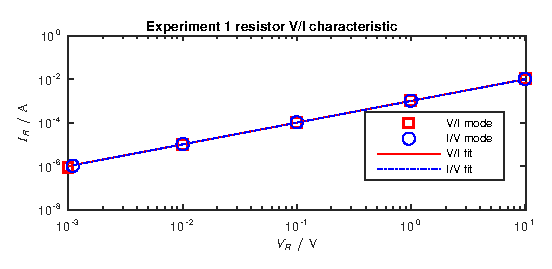
\includegraphics[width=\textwidth]{manual-measure.eps}
    \caption{Manual measurement of the I-V characteristics of the resistor. }
    \label{fig:manual-measure}
\end{figure}
\section{Manual Data Acquisition}
We performed 5 measurements in both V/I and I/V mode using the 236 SMU. In V/I mode we 
performed order of magnitude steps from 0.0001 V to 10 V, and in I/V mode from 1\(\mu\)A to
10mA. Fig.~\ref{fig:manual-measure} shows the I-V characteristics we obtained. In a V/I
plot, the slope of the graph is the inverse of the resistance. Using linear regression forced
through zero, we obtain
\begin{equation*}
    R_{V/I} = 991.97\Omega, \quad R_{I/V} = 993.94 \Omega
\end{equation*}
Using the resistors color code we identified it as a 1k\(\Omega\) 1\% tolerance resistor, placing
the found resistance value within its specification.

Using single measurements at the high end of the scale, we find 
\begin{equation*}
    R_{V/I} = 992.06\Omega,\quad R_{I/V} = 994.00\Omega
\end{equation*}

And using single measurements at the low end of the scale
\begin{equation*}
    R_{V/I} = 1111.11\Omega, \quad R_{I/V} = 1100.00\Omega
\end{equation*}
These values are very far from the tolerance value of the resistor and far outside
of the combined source and measurement error range. The large error is most likely
due to us dropping the two least significant digits in the measurement because they did
not settle.

While the I/V mode measurements yield a result closer to the nominal value of the resistor,
but values are within the tolerance range and we therefore cannot conclude which mode is more
accurate based on this, assuming of course we would trust the resistor manufacturer not to 
ship resistors outside of their tolerance range.

Instead we calculate the maximum combined source/measurement error in both modes and conclude
that V/I mode is more precise.

\section{An Exponential Transfer Function}
\begin{figure}
    \center
    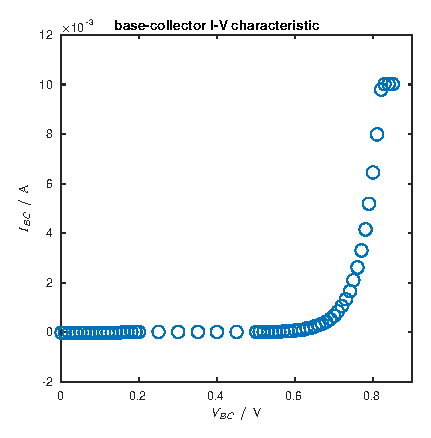
\includegraphics[width=0.5\textwidth]{ivc.eps}
    \caption{I-V characteristic of the base-collector PN junction. The exponentional part of the curve
    starts just after 0.2 V. The compliance limit of 10 mA is hit at 0.81V.}
    \label{fig:ivc}
\end{figure}

\begin{figure}
    \center
    \begin{subfigure}{.8\textwidth}
    \center
        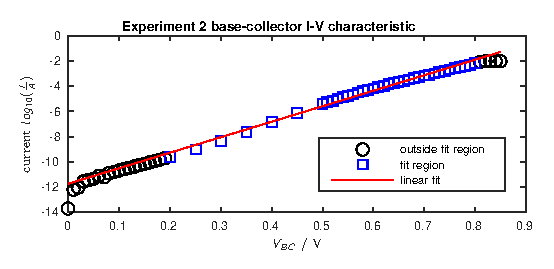
\includegraphics[width=\textwidth]{log10ivc.eps}
        \caption{}
    \end{subfigure}
    
    \begin{subfigure}{.8\textwidth}
    \center
        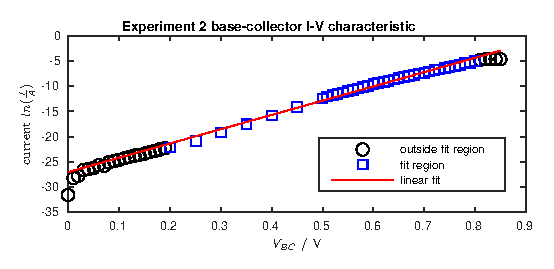
\includegraphics[width=\textwidth]{lnivc.eps}
        \caption{}
    \end{subfigure}
    \caption{I-V characteric of the base-collector PN junction on semilog plots in base 10 (a) and base \(e\) (b). 
    The square measurement points were used to fit a linear function. Fewer data points were gathered in the \(0.2-0.5\) V
range to save measurement time. The flattening of the curve at \(0.80\) V is a result of our 10 mA current limit being met.}
\label{fig:ivclog}
\end{figure}

We used the Matlab function \texttt{iv()} to gather data points from the pico-ampere to the milli-ampere current range, 
by sweeping from 0 V to 0.85 V in steps of 0.01 V between 0-0.2 V and 0.5-0.8 V, and in steps of 0.05 V between 0.2-0.5 V.

\subsection{Over what range of currents/voltages does the diode behave exponentionally?}

Fig.~\ref{fig:ivc} shows the I-V characteristic of the base-collector junction. The exponentional part of the curve begins
shortly before 0.2 V and we will use the 0.2-0.8 V range when calculating the slope of the exponentional. The exponential
curve will continue beyond 0.8 V, but we cannot follow it since we hit the current limit of 10 mA.

\subsection{How small a current were you able to measure confidently?}
Figures~\ref{fig:ivclog} and~\ref{fig:ivelog} show semilog plots of the I-V characteristics for the base-collector and
base-emitter junctions respectively. The measurements begin to look unreliable, because of noise, below a few pico-amperes.

\subsection{What is the slope of the exponential, expressed in mV/e-fold and mV/decade of current?}
We fit a linear function to the data points between 0.2-0.8 V in Figures~\ref{fig:ivclog} and~\ref{fig:ivelog}. 
The slope of the exponential in mV/decade is then the inverse of the slope of the linear function obtained in 
the base 10 log plots. Likewise, the slope of the exponentional in mV/e-fold is the inverse of the linear function
slope obtained in the base \(e\) log plots.

We obtain the following slopes:
\begin{align*}
    \frac{dV_{BC}}{dI_{BC}} &= 35.34 \frac{\text{mV}}{\text{e-fold}} = 81.38 \frac{\text{mV}}{\text{decade}} \\
    \frac{dV_{BE}}{dI_{BE}} &= 30.35 \frac{\text{mV}}{\text{e-fold}} = 69.88 \frac{\text{mV}}{\text{decade}}
\end{align*}


\begin{figure}
    \center
    \begin{subfigure}{.8\textwidth}
    \center
        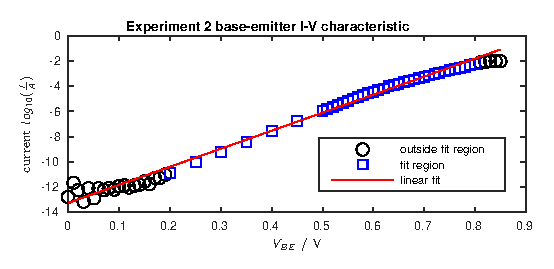
\includegraphics[width=\textwidth]{log10ive.eps}
    \caption{}
    \end{subfigure}
    
    \begin{subfigure}{.8\textwidth}
    \center
        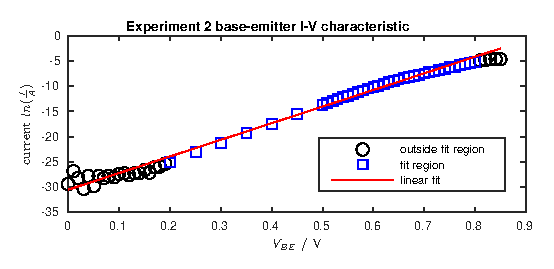
\includegraphics[width=\textwidth]{lnive.eps}
    \caption{}
    \end{subfigure}
    \caption{I-V characteric of the base-emitter PN junction on semilog plots in base 10 (a) and base \(e\) (b). 
    The square measurement points were used to fit a linear function. Fewer data points were gathered in the \(0.2-0.5\) V
range to save measurement time. The flattening of the curve at \(0.80\) V is a result of our 10 mA current limit being met.}
\label{fig:ivelog}
\end{figure}

We are measuring the PN-junctions in the 2N3904 BJT while leaving the terminal not in use floating. A single PN-junction is a
diode, and for a non-ideal diode, the current though the diode is given by 
\begin{equation*}
    I_D = I_0\left(e^{\frac{qV}{nkT}}-1\right)
\end{equation*}
Where \(k\) is Boltzmann's constant, \(q\) is the elementary charge and \(n\) is the ideality factor of the diode.

If the diode temperature was approximately the same as the temperature of the lab at the time of the experiment, say \(\sim295K\),
the slope of the exponential in mV/e-fold will be 
\begin{equation*}
    \frac{dV_{BE}}{dI_{BE}} = 25.42n \frac{\text{mV}}{\text{e-fold}}
\end{equation*}
Meaning that our ideality factors for the base-collector and base-emitter junctions are
\begin{align*}
    n_{BC} &= \frac{{35.34 \frac{mV}{\text{e-fold}}}}{25.42\frac{mV}{\text{e-fold}}} = 1.39 \\
    n_{BE} &= \frac{{30.35 \frac{mV}{\text{e-fold}}}}{25.42\frac{mV}{\text{e-fold}}} = 1.19
\end{align*}
\end{document}
